% !TeX spellcheck = en_US
\documentclass[./main.tex]{subfiles}
\begin{document}
	\subsection{Mobile app architecture}
	% TODO ori change this accordingly to what do we have to show.
	In this subsection, the decisions regarding the architecture of the mobile app will
	be explained, but not those that regard the user experience of the mobile. This 
	will be explained in more detail at  \ref{sec:views}.\\
	\\
	As it was said in the former spring, the mobile application development is still done with Flutter. The reason of why the app is implemented by flutter and not other frameworks, as Android or React Native,
	will be explained in
	 \ref{sec:flutter}.
	Then, it will be introduced the Redux for the state management	of the app  in \ref{sec:redux}. Finally, the changes of the mobile application architecture for this sprint will be in \ref{sec:flutter-changes}.
	\subsubsection{Flutter}
	\label{sec:flutter}
	Flutter is a multiplatform framework aiming to become a standard for building apps that have to work on either Android or iOS, as well as the web, desktop, and embedded operative systems. \\
	\\
	As a tool, it has been proven that it can build more resilient and optimized apps than its counterparts, like React Native, while still being multiplatform. Even though it was taught how to work with native Android Applications, it was decided to choose this tool against it as the team had already some experience with it.\\
	\\
	Even if the framework is young, the community behind flutter is active and has several repositories that have some application examples, as well as a libraries showcase that has and will help the development of the app.
	\subsubsection{Redux}\label{sec:redux>}
	State management in applications is a hot topic, and although both frameworks used by the clients in this project have some way to implement it, it was preferred to use a third-party option that is well consolidated, easy to use, and easy to manage.\\
	\\
	Redux is an abstraction that provides a way to implement easier a reactive pattern, that is, instead of having the typical Model-View-Controller, it has a way of drawing a State, the buttons can launch actions, that is taken by reducers along the actual state, and return the
	next state, as shown at \ref{fig:redux}.\\
	\\
	\begin{figure}[H]
		\centering
		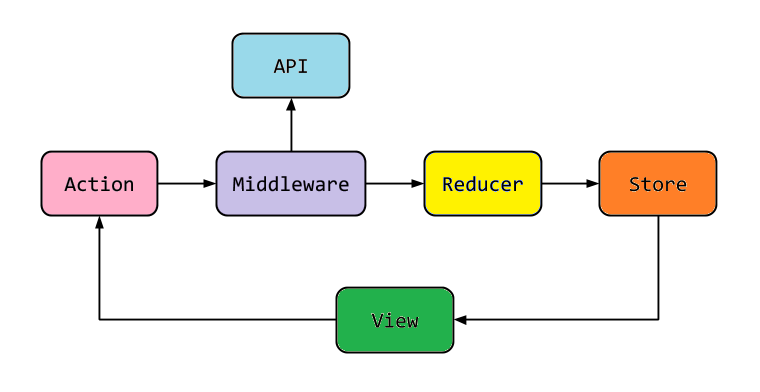
\includegraphics[width=0.8\textwidth]{img/redux.png}
		\caption{Redux Diagram.}
		\label{fig:redux}
	\end{figure}
	This makes the components stateless, which makes it easier to work with them and provides a way of mesmerizing them so they aren't computed that many times, making them faster than their counterparts. 
	\\
	\\
	This also helps to have a way of monitoring the changes that the state has suffered, as you can keep the states and the actions in a list for debugging, so it can be traced easily the changes. This adds when you have to have a shared object that won't be modified easily, but has to be read by most of the components, as an API token or a theme object. In order to do that, the different functionalities of the mobile application have been splitted and sorted. Therefore, it has been created in every package a \texttt{store} and \texttt{action} dart files which contain all the logic of the management of the store globally.
	\\
	\\
	Finally, as it was also used in the web applications, it makes the team be able to change quickly between the two frameworks, as the most difficult part is done the same way.
	\subsubsection{Service Package}
	Regarding the connection to the backend, it has been created a package to manage all the data received and turning the data transfer objects into data models, which interacts to the logic and design of the application. In \textit{Figure \ref{fig:redux}}, it can be seen how this package is connected through the app.
	\subsubsection{Asynchronous Actions}
	In order to connect to the backend API, it is compulsory to use asynchronous actions. Even though, Redux only provides pure functions dispatches and the state can not wait for asynchronous calls. In order to do that, it was needed a higher layer to do this communication. A good way is implementing a middleware between dispatching and reducing the action to a new state.
	\\
	\\
	The middleware would catch the new middleware actions, which could be asynchronous, and then dispatches the other logical actions. A library called \texttt{ReduxThunk} was imported to make the middleware easier. The thunk actions provides making asynchronous calls returning the store as the effect of the action instead of the state.
	\\
	\\
	A clear example is \texttt{clearSearchAndReload}, which you can dispatch lower level actions and do asynchronous calls inside the actions.
	\begin{verbatim}
	ThunkAction<AppState> clearSearchAndReload() {
	    return (Store<AppState> store) async {
	        store.dispatch(ClearSearch());
	        final HashMap<int, Product> products =
	        await store.state.commedMiddleware.getProducts();
	        store.dispatch(SetProductList(products));
	    };
	}
	\end{verbatim}
	\subsubsection{WebSocketChannel}
	The part of connecting to the WebSockets in order to send and receive messages without doing gets and posts is more or less trivial. The library \texttt{}. One of the most challenges in this was connecting correctly and getting the messages correctly through the channel and then, reload the state and dispatching the store to display the new information. The library used for connecting to the WebSocket is called \texttt{web\_socket\_channel}.
	
\end{document}